\chapter{并发布鲁姆过滤器设计}
%引子
% 对于海量数据处理业务,通常需要建立索引数据结构来帮助查询,快速判断数据记录是否存在,过滤器(filter)能够很好的满足构建索引数据结构的要求。
查找或判断一个元素是否存在于一个指定集合中,这是计算机科学中一个基本问题。
通常会采用线性表(数组或链表)、树(二叉树、堆、红黑树、 B+/B-/B*树)等数据结构存储所有元素,对数据进行排序和查找。
这里的查找时间复杂性通常都是O(N)或O(log(N))。
如果集合元素非常庞大,不仅降低了查找的效率,同时对内存空间的需求也非常大。

在网络安全领域有一个简单的应用场景:判断URL是否链接到存在安全隐患的网站。
用户在浏览器内输入URL,浏览器需要判断该URL是否是恶意的,它将该URL与本地缓存的URL进行匹配,如果匹配失败,则说明该URL是安全的链接可以正常访问;否则,说明该URL可能存在安全隐患。
此时,提交请求给远程客户端进行验证,并警告用户该URL存在风险。
在这个应用场景中,如果缓存的URL数量很少,那么使用上述的数据结构都可以达到较高的查找效率,同时对内存空间的要求也不高。
假设现在需要缓存的URL的数量为10亿条(这在当前是很常见的一个数量级),每条URL的大小为8个字节,那么存储所有的URL大约需要8 GB的内存。
使用哈希表是一种可能的解决方案.哈希表的查询时间复杂度为O(1),可以节省查找的时间,但是没有降低对内存的需求。

事实上,除非有特别的需求,否者判断元素是否在一个指定集合内,并不需要把所有元素的原始信息都保存下来,而只需要保存该元素的“存在状态”,存储存在状态只需要几个bit。
使用哈希函数可以将元素映射成位数组中的一个点,采用k个哈希函数将元素映射成k个点。
这样,经过映射之后,查找元素是否存在时只需看看特定的几个位点的值就能判断某个元素是否存在于集合当中,如果k个位置都为1,则说明该元素可能存在,如果有1个位置上为0,则可以肯定该元素不存在。
这样不仅可大大缩减内存空间,查找速度非常
这就是布鲁姆过滤器(Bloom Filter)的基本思想。
它的名字源自其发明者Burton.H Bloom\cite{bloom1970space}。
布鲁姆过滤器最初应用于拼写检查和数据库系统。
但是,随着互联网的爆炸式发展,海量数据中快速检索目标数据的需求使得布鲁姆过滤器的应用焕发新生,涌现出新的应用和变种\cite{bender2012don,bonomi2006improved,song2005fast,yu2009buffalo}。

\section{布鲁姆过滤器}

\subsection{基本原理}
布鲁姆过滤器使用位数组表示元素集合S,并使用k个哈希函数(h$_1$, h$_2$, ..., h$_k$)来对元素进行位映射。
初始状态下的布鲁姆过滤器是一个包含m位的位数组,每一位都置0,图~\ref{fig:bf}(a)所示为m = 12的布鲁姆过滤器。
当需要将集合S中的n个元素x$_1$,x$_2$, ... x$_n$用位数组表示时,对该元素分别使用k个相互独立哈希函数进行计算,得到位数组上k个位置的索引值,随后将映射到位数组的相应位置1。
值得注意的是,如果一个位置被多次置为1,只有第一次的置位是有效的。
图~\ref{fig:bf}(b)表示k = 3时,将元素映射到位数组的过程,其中元素x$_1$和x$_2$都对第5位置位。
图~\ref{fig:bf}(c)表示判断元素y$_i$(i = 1,2, ..., n)是否属于集合。
与插入过程类似,同样先对y进行k次哈希,如果计算得到的索引值对应的位上有任何一位为0则表示y元素绝对不存在于集合中,只有当所有映射位均为1时才表示该元素\textbf{有可能}存在于集合当中。
\begin{figure}[htbp]
\centering
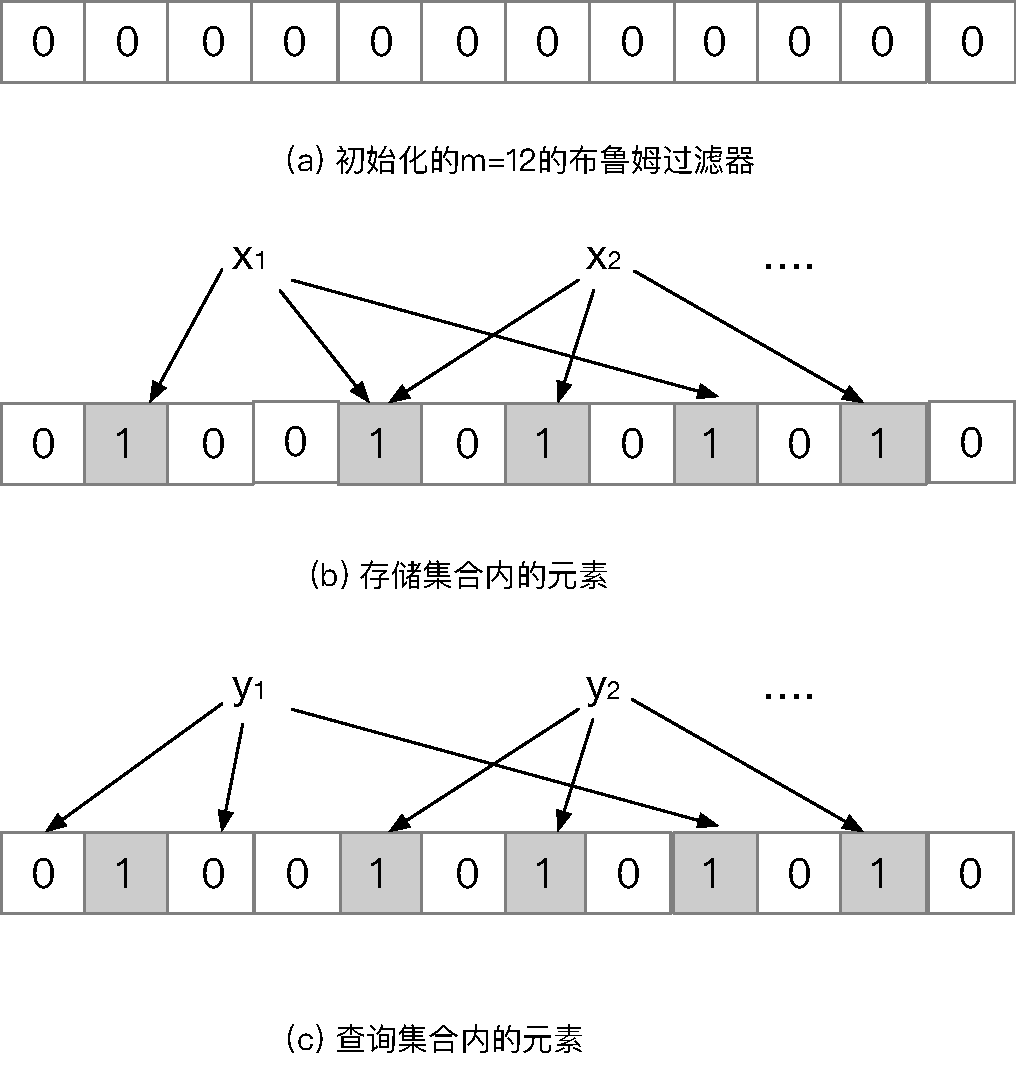
\includegraphics[width=0.65\textwidth]{bloomfilter}
\caption{布鲁姆过滤器}\label{fig:bf}
\end{figure}
换句话说,如果布鲁姆过滤器判断一个元素不在集合中,那肯定就不存在;而如果判断存在,则不一定存在,下文将对这种不一定存在的原因进行说明。
这种不能确定元素一定存在的问题是由哈希函数可能发生碰撞的特性所决定的。
这个错误率可调整位数组大小或者哈希函数个数进行控制。
由此可见,布鲁姆过滤器的高效是以一定的误报为代价的,它通过容忍一定的错误发生的概率换取存储空间的极大节省。
布鲁姆过滤器不适合那些“零错误”的应用场合。

标准的布鲁姆过滤器不支持删除操作。
原因很简单,考虑在图~\ref{fig:bf}(b)中删除元素x$_2$,意味着将位数组内的第5、7、11位置0,此时如果查询x$_1$会发现也不存在,因为它对应的第5位上的值在删除x$_2$时被置0了。

标准布鲁姆过滤器的实现中有几个重要参数:误判率\begin{math}\epsilon\end{math}、负载因子\begin{math}\alpha\end{math}、哈希函数的个数k、位数组大小m和集合中元素的个数n。下面将对这些参数进行推导,以确定实现标准布鲁姆过滤器的参数选取原则。

\subsection{误判率估计}
在进行正式的误判率估计前先明确几个定义和重要的参数:
\begin{definition}
	假阳性(false positives)也叫误判是指当前元素不在集合内,但由于哈希冲突的缘故存在其它元素被映射到部分相同bit位上,从而有一定的概率导致在判定该元素时认定其对应的所有位置都为1,从而判定其在集合内,造成一次误判。这个概率本文称为误判率,误判率用\begin{math}\epsilon\end{math}表示。
\end{definition}

\begin{definition}
	假阴性(false negatives),也叫漏报,是指在位数组内删除某个元素,导致该元素对应的比特位置0,造成本来存在的元素会被漏报成不存在。
\end{definition}

\begin{definition}
	负载因子是指集合中的元素的个数\textit{n},布鲁姆过滤器位数组的位数\textit{m}之间的比值,它用\begin{math} \alpha \end{math}表示,其中\begin{math} \alpha  = {n/m} \end{math}。当\begin{math} \alpha \end{math}为0时,表示布鲁姆过滤器为空,\begin{math} \alpha \end{math}为1表示布鲁姆过滤器满载。
\end{definition}

下面进行误判率\begin{math}\epsilon\end{math}的推算.
首先假设布鲁姆过滤器中使用的k个哈希函数的计算结果都是均匀分布的,即每个元素都等概率地被哈希到m个bit位上的任何一个,与其他元素被哈希到的位置无关。
则对某一特定bit位在一个元素由特定哈希函数插入时没有被置位为1的概率p$_1$为:
\begin{equation}
p_1 = 1-\frac{1}{m}
\end{equation}
则k个哈希函数中都没有一个对其置位的概率p$_2$:
\begin{equation}
p_2 = {p_1}^k
\end{equation}
如果插入n(\begin{math}n\leqslant m\end{math})个元素,但都未对其置位的概率p$_3$:
\begin{equation}
p_3 = {p_2}^n = {p_1}^{kn}
\end{equation}
则此位被置位的概率p$_4$为:
\begin{equation}
p_4 = 1 - \left(1 - \frac{1}{m}\right)^{kn}
\label{equ:alpha}
\end{equation}
现在考虑判定阶段,若对应某个判定元素的k个位全部置位为1,则可判定其在集合中。因此将某元素误判的概率为:
\begin{equation}
\epsilon = \left(1 - \left(1 - \frac{1}{m}\right)^{kn}\right)^k
\label{equ:epsilon}
\end{equation}


由
\begin{math} \left(1 + x\right)^{\frac{1}{x}} \thickapprox e \end{math}
可知,但m很大时,满足
\begin{math}-\frac{1}{m} \to 0\end{math},
可将公式\ref{equ:alpha}转化为:
\begin{equation}
\epsilon = \left(1 - \left(1 - \frac{1}{m}\right)^{{-m}\frac{-kn}{m}}\right)^k \thickapprox \left(1 - e^{-\frac{nk}{m}}\right)^k
\label{equ:beta}
\end{equation}
由公式\ref{equ:beta}可以初步断定\begin{math}\epsilon\end{math}与元素的个数n和位数组的长度m决定,增大n或者减小m都会导致\begin{math}\epsilon\end{math}的升高。这种计算方法不严格,因为前面假设哈希函数和散列后值的分布是相互独立的。
但是,这个假设随着m和n的增大误判率更接近真实的误判率。
Mitzenmacher证明无假设情况下的误判率的期望值相同\cite{mitzenmacher2002compressed}。

\subsection{最优哈希函数个数}
\label{sec:num_hashf}
哈希函数的选择对于布鲁姆过滤器的性能以及空间利用率都有至关重要的作用。
对于选取什么样的哈希函数已经在前文中有过介绍,这里不再缀述。
而对于哈希函数的个数,直观的认为越多越好。实际上,哈希函数越多,用于表达集合中每一个元素所需要的位数就越多,这与布鲁姆过滤器用较低的误判率换取空间的高效利用的初衷相悖。那么哈希函数的个数应该满足什么条件才能有最佳性能呢?

下面推导对给定的\begin{math}\alpha\end{math},k满足什么条件可以使\begin{math}\epsilon\end{math}最小化。

令:
\begin{equation}
f\left(k\right) = \left(1 - e^{-\frac{nk}{m}}\right)^k 
\end{equation}

取 b = e$^{n/m}$,得:
\begin{equation}
f\left(k\right) = \left(1 - b^{-k}\right)^k 
\end{equation}

两边取对数得: 
\begin{equation}
lnf\left(k\right) = k\ast ln\left(1 - b^{-k}\right)
\end{equation}

函数两边对k求导得:
\begin{equation}
\frac{1}{f\left(k\right)} f'\left(k\right) = ln\left(1 - b^{-k}\right) + k \frac{b^{-k}\ast lnb}{1 - b^{-k}} 
\label{equ:fk}
\end{equation}

对式~\ref{equ:fk}右边求最值。

令:
\begin{equation}
\begin{split}
\frac{1}{f\left(k\right)}f'\left(k\right) = ln\left(1 - b^{-k}\right) + k \frac{b^{-k}\ast lnb}{1 - b^{-k}} = 0 \\
\Rightarrow \left(1 - b^{-k}\right) ln\left(1 - b^{-k}\right) = -k\ast b^{-k}lnb \\
\Rightarrow 1 - b^{-k} = b^{-k} \\
\Rightarrow e{-\frac{kn}{m}} = \frac{1}{2}\\
\Rightarrow k = ln2\ast \frac{m}{n} \thickapprox 0.7\frac{m}{n}
\end{split}
\end{equation}
因此,对于固定的\begin{math}\alpha\end{math},当\begin{math}k = 0.7\frac{m}{n}\end{math}时具有最低的误判率,此时\begin{math}\epsilon\end{math}等于:
\begin{equation}
\left(1 - \frac{1}{2}\right)^k = 2^{-ln2{m}{n}} \thickapprox 0.62\frac{m}{n}
\end{equation}

\subsection{最优位数组长度}
下面进行给定一定的误判率上限,布鲁姆过滤器至少需要多少位才能表示全集中任意的x个元素的集合。
假设全集中元素的个数为n,最大误判率为\begin{math}\epsilon\end{math}。以此为前提展开对位数组大小的推导。

假设S$_n$为全集中任取n个元素的集合,B是表示S$_n$的位数组。
那么对于集合S$_n$中任意一个元素x,在B中查询x都能得到肯定的结果,即B能够接受x。
显然,由于布鲁姆过滤器引入允许误判,B能够接受的不仅仅是S$_n$中的元素,它还允许最多\begin{math}\epsilon\end{math}*(u - n)个误报。因此,对于一个确定的位数组来说,它能够接受总共n + \begin{math}\epsilon\end{math}*(u - n)个元素。在n + \begin{math}\epsilon\end{math}*(u - n)个元素中,B真正表示的只有其中n个,所以一个确定的位数组可以表示:
\begin{equation}
\binom{n + \epsilon *\left(u - n\right)}{n}
\end{equation}
个集合。m位的位数组一共有2$^m$个不同的组合,可以进一步推导m位的位数组可以表示:
\begin{equation}
2^m\binom{n + \epsilon *\left(u - n\right)}{n}
\end{equation}
个集合。全集中包含n个元素的子集总共有:
\begin{equation}
\binom{u}{n}
\end{equation}
个。因此,要让布鲁姆过滤器的位数组大小能够满足所有包含n个元素的子集,必须满足:
\begin{equation}
2^m\binom{n + \epsilon *\left(u - n\right)}{n} \geq \binom{u}{n}
\end{equation}
即m需要满足:
\begin{equation}
m \geq log_2\frac{\binom{u}{n}}{\binom{n + \epsilon *\left(u - n\right)}{n}} \geq log_2\frac{\binom{u}{n}}{\binom{\epsilon u}{n}} \thickapprox log_2\epsilon^{-n} = n log_2\left(\frac{1}{\epsilon}\right)
\label{equ:bfm}
\end{equation}
式~\ref{equ:bfm}中近似相等有个重要的前提条件:n远小于\begin{math}\epsilon\end{math}u,这个前提在实际的问题中也是常见的。
根据式~\ref{equ:bfm}中的不等式,得到如下结论:在误判率上限为\begin{math}\epsilon\end{math}的情况下,m至少要等于\textit{n}log$_2$(1/\begin{math}\epsilon\end{math})才能表示任意n个元素的集合。

在本章~\ref{sec:num_hashf}中推导出哈希函数的个数k等于\begin{math}k = 0.7\frac{m}{n}\end{math}时可以得到最小误判率,此时的误判率为\begin{math}(\frac{1}{2})^{0.7\frac{m}{n}}\end{math}。
令\begin{math}(\frac{1}{2})^{0.7\frac{m}{n}} \leq \epsilon \end{math},可以进一步推导:
\begin{equation}
m \geq n\frac{log_2(\frac{1}{\epsilon})}{ln2} = nlog_2e\ast log_2(\frac{1}{\epsilon}) \thickapprox 1.44\textit{n}log_2(\frac{1}{\epsilon})
\label{equ:bfm2}
\end{equation}

式~\ref{equ:bfm2}说明当k取到最优值时,要保证误判率不超过给定的上限\begin{math}\epsilon\end{math},m至少要取到最小值的1.44倍。
可以验证,当给定\begin{math}\epsilon\end{math} = 0.01时,存储每个元素需要9.6比特。
而将\begin{math}\epsilon\end{math} = 0.001时,每个元素需要额外的增加4.8比特。
所以,在实际的应用中,对于误判的容忍度不同,要求误判率越低,则存储每个元素需要的比特位越多,相同容量下存储的元素个数就越少。

\section{Cuckoo过滤器}
传统的布鲁姆过滤器的空间效率高,对插入和查询元素的处理也相当快。
但是它也存在缺陷——存在一定的误报率,不支持元素的删除操作。
消除误报率除非能实现没有碰撞的哈希函数,但是不发生碰撞的哈希函数至今没有被设计出来。
研究人员能做的就是尽量选择均匀的哈希函数,并且借助一些数据结构的特性有效的对碰撞进行处理。
而在上一节的中介绍到误判率每缩小到原来的十分之一,用于表示元素的比特数至少要增加4.8。
另外,实现元素删除操作的一个方法是引入计数器,将每个比特位都扩张成一个计数值,降低了空间效率。
为了支持对元素的删除操作,出现了很多标准布鲁姆过滤器的扩展版本\cite{bender2012don,bonomi2006improved,fan2000summary}。
所以,布鲁姆过滤器实现更低的误判率和实现删除操作都需要牺牲一定的空间效率。

为了解决上述问题,本文引入一种新的数据结构——Cuckoo过滤器。
它既可以确保该元素存在的必然性,即将“可能存在”变成“一定存在”;
又支持动态的对元素的插入和删除,而不会造成漏报。

\subsection{Cuckoo过滤器算法描述}
% 近几年,有研究人员将Cuckoo哈希表应用于集合元素查询。为了支持事务内存,Sanchez\cite{sanchez2007implementing}等人提出将每条事务的内存地址的读/写集存入到Cuckoo哈希表中,当哈希表内的元素达到饱和时,将其转化为布鲁姆过滤器。
为了支持动态的插入和删除元素,Cuckoo过滤器采用的是一种称为\textbf{不完整键值(partial-key)} Cuckoo哈希的技术。
Cuckoo过滤器是标准Cuckoo哈希表在集合元素查询算法领域的应用。
在前面的章节中已经对Cuckoo哈希表的基本原理和概念有过详细介绍(\textcolor{red}{第~\ref{sec:XX}节}),这里不再赘述。
仅对与在这一部分密切相关的术语进行重申。
Cuckoo的数据结构与Cuckoo哈希表相同,其基本单元称为\textbf{实体}(entry),不同的是每一个实体内存储的不是完整的键值,而是根据键值进行提取后的\textbf{指纹}(fingerprint)~\cite{memc3},用f表示。
哈希表由存储了多个实体的\textbf{桶}(bucket)数组构成。
\textbf{条目}(item)是指键值对。
本小节对Cuckoo过滤器的查询、插入和删除操作的实现进行介绍。

\subsubsection{插入操作}
在标准Cuckoo哈希表中,在哈希表中插入新的条目时需要以某种方式读取原本存储于哈希表内的条目,以便在发生踢出原始条目时确定将该条目安置在哪个位置上。
但是,对于只存储了指纹的Cuckoo过滤器而言,它无法根据原始条目的键计算出旧键迁移到哪个位置。
这里引入不完整键Cuckoo哈希算法来解决无法根据指纹信息定位旧键迁移位置的问题。对任意的条目\textit{x},使用公式~\ref{equ:ckf}计算其两个备选哈希桶的索引值:
\begin{equation}
\begin{split}
h_1\left(x\right) &= hash\left(x\right) \\
% \label{equ:ckf1}
% \end{equation}
% \begin{equation}
h_2(x) &= h_1(x)\bigoplus hash(\text{x的指纹信息})
\end{split}
\label{equ:ckf}
\end{equation}

式~\ref{equ:ckf}的异或操作有一个重要的特性:h$_1$(x)可以通过h$_2$(x)和指纹信息用同样的公式推算出来。
即就是说,替换编号为\textit{i}的哈希桶中的旧键(不论\textit{i}对应的是h$_1$还是h$_2$),都可以通过当前桶编号\textit{i}以及存储在该桶内的指纹直接计算出旧键的备选哈希桶的编号\textit{j},计算过程如式~\ref{equ:ckf2}所示。
\begin{equation}
 % \begin{split}
j = i \bigoplus hash(\text{指纹信息})
%
% \end{split}
\end{equation}
因此,在进行插入操作时,不用检索目标哈希桶内存储的条目的完整信息,只需要存储在哈希表中的指纹信息。

另外,为了使众条目在哈希表中均匀分布,在与索引值进行异或运算之前,指纹信息已经进行过哈希运算。
当指纹信息远小于哈希表的大小时,如果直接使用索引值与未经哈希的指纹信息进行异或运算推算接纳被踢出条目的哈希桶的位置,那么接纳被踢出的条目哈希桶与原来的哈希桶在位置上很近。
下面举例说明。
使用8比特的指纹信息时,接纳从\textit{i}中被踢出的条目的哈希桶的位置距离\textit{i}的最大距离为2$^8$。
这时因为在进行异或运算时,会选取索引值的低8位进行运算,而高8位保持不变。
对指纹信息进行哈希能够确保这些条目尽量分散在哈希表的不同位置,从而可以避免哈希碰撞,提高哈希表的空间利用率。

\SetKwProg{Fn}{Function}{}{}
\begin{algorithm}[htbp]
\SetAlgoLined
\Fn{Insert(x)}{}{
f = fingerprint(x)\\
i1 = hash(x)\\
i2 = i1\begin{math}\bigoplus\end{math}hash(f) \\
\If{\text{桶i1或i2内有空闲实体}}{
	{将f存入i1或i2}\\
	\Return $Done$;
	}

\tcc{当前桶内没有空闲位置}
i = rand(i1, i2) \\% \tcc{随机的从i1、i2中选取一个桶} \\
\For{$n=0$ \KwTo $MaxNumKicks - 1$}{
	{从bucket[i]中随机的选择一个实体e}\\
	{将新插入条目的指纹信息与e的指纹信息交换}\\
	i = i\begin{math}\bigoplus\end{math}hash(f)\\
	\If{\text{bucket[i]有空闲实体}}{
		{将f存储到bucket[i]}\\
		\Return $Done$
	}
}
\tcc{哈希表饱和}
\Return $Failure$
}
\caption{Cuckoo过滤器插入操作}
\label{algo:ckf_insert}
\end{algorithm}

算法~\ref{algo:ckf_insert}给出了使用不完整键Cuckoo哈希方法对Cuckoo过滤器动态插入元素的过程。
指纹信息的长度小于h$_1$和h$_2$的长度造成的后果有两个方面:
\textbf{第一},通过公式~\ref{equ:ckf}计算出的\textit{(h$_1$, h$_2$)}的组合的总数会远远小于使用完整的哈希值计算得到的组合的数量,这将导致哈希碰撞更严重;
\textbf{第二},允许插入两个具有相同指纹的条目\textit{x}和\textit{y},在一个哈希桶内可能出现多个相同的指纹信息是合法的。
但是如果相同的指纹信息的数量超过2b(b为哈希桶的大小)时,存储其指纹信息的哈希桶会过载。
解决哈希桶过载的途径有多种。
\begin{itemize}
	\item 第一,也是最简单的方法——不实现过滤器删除元素操作,这样每条指纹信息都只需要存储一份副本。但这显然与Cuckoo过滤器的设计初衷不符。
	\item 第二,引入适当的空间开销在哈希桶内加入计数器,进行插入/删除操作时适当的自增/自减。
	\item 第三,将原始的键存储在其他位置(可以是访存速度较慢的外存上),这样可以在插入时查看该记录,防止重复插入。
	但是如果哈希桶内已经存在匹配的实体,则插入的速度相对较慢。
\end{itemize}	

\subsubsection{删除操作}
在标准的布鲁姆过滤器中删除条目需要对整个过滤器进行重建,引起惊人的性能开销。所以标准布鲁姆过滤器不支持删除操作。
而将布鲁姆过滤器的比特位扩展成计数值的方法需要耗费3-4倍的空间开销。
Cuckoo过滤器可以直接从过滤器中移除相关条目的指纹完成删除操作。
有关Cuckoo过滤器的删除过程如算法~\ref{algo:ckf_delete}所示。
\SetKwProg{Fn}{Function}{}{}
\begin{algorithm}[htbp]
\SetAlgoLined
\Fn{Delete(x)}{}{
	f = fingerprint(x) \\
	i1 = hash(x); \\
	i2 = i1\begin{math}\bigoplus\end{math}hash(f) \\
	\If{\text{bucket[i1]或bucket[i2]中含有f}}{
		{从当前bucket内删除f的一个副本}\\
		\Return $True$
	}

	\Return $False$
}
\caption{Cuckoo过滤器的删除操作}
\label{algo:ckf_delete}
\end{algorithm}

相比当前一些支持删除操作的布鲁姆过滤器的扩展版本,比如\textit{d-left}计数过滤器,熵过滤器的实现,Cuckoo过滤器的删除操作十分简单。
对于一个需要删除的条目,Cuckoo过滤器首先根据索引值在桶内进行查找;如果在任意的桶内有匹配的指纹信息,则删除该桶内的指纹信息的一个副本。

在删除某个条目后,不需要对这个实体进行清理。
这样可以避免在同一个桶内存有两个具有相同指纹信息的条目时的“误删”。
假设条目\textit{x}和\textit{y}都映射到了桶\textit{i}$_1$内,并且具有相同的指纹信息\textit{f}。
因为\textit{i}$_2$ = \textit{i}$_1$\begin{math}\bigoplus\end{math}hash(f),所以它们同样能够保存在桶\textit{i}$_2$内.
在删除\textit{x}时,不用考虑删除的指纹信息的副本是在插入\textit{x}还是\textit{y}是添加的。
删除\textit{x}后,在桶\textit{i}$_1$、\textit{i}$_2$中\textit{y}仍然可以被查询到。

值得注意的是,在上面的例子中删除条目\textit{x}之后,过滤器的误判行为仍然存在。
过滤器中的\textit{y}会在查询\textit{x}时误报,因为两者具有相同的桶索引值和指纹信息。
误判行为仍然在近似集合元素查询数据结构接受的范围之内,误判率也仍然满足\begin{math}\epsilon\end{math}的上界约束条件。

安全的删除条目有一个前提条件:被删除的\textit{x}必须是已经插入到了过滤器中的条目。
否则的话,有可能造成过滤器内恰好就有相同指纹信息的条目。
这条原则不仅是对Cuckoo过滤器,同样对其他支持删除操作的过滤器也适用。

\subsubsection{查询操作}
\SetKwProg{Fn}{Function}{}{}
\begin{algorithm}[htbp]
\SetAlgoLined
\Fn{Lookup(x)}{}{
	f = fingerprint(x) \\
	i1 = hash(x); \\
	i2 = i1\begin{math}\bigoplus\end{math}hash(f) \\
	\If{\text{bucket[i1]或bucket[i2]中含有f}}{
		\Return $True$
	}

	\Return $False$
}
\caption{Cuckoo过滤器查询操作}
\label{algo:ckf_lookup}
\end{algorithm}
Cuckoo过滤器的查询操作相对简单。算法~\ref{algo:ckf_lookup}对这个过程做了简单描述。
对于给定的条目\textit{x},首先计算其指纹并根据公式~\ref{equ:ckf}计算出它的两个哈希桶的索引值。
然后遍历这些哈希桶:如果在任何一个桶内找到了\textit{x}的指纹,则返回True。否则返回False。
值得注意的是,只要哈希桶不发生溢出,就能确保不存在任何误报。

\subsection{Cuckoo过滤器的参数}
\subsubsection{指纹信息的长度}

\subsection{最优哈希桶大小}
\section{并发Cuckoo过滤器}
\subsection{}
\subsection{}
\subsection{}

\section{本章小结}